\chapter{\Uid{}s}
\label{sec:uid}

\begin{figure}[H]
\center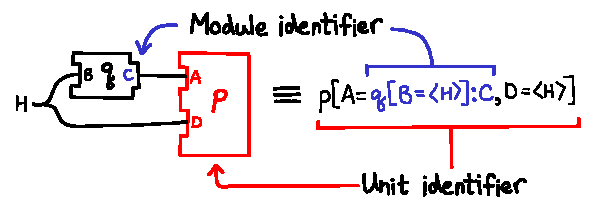
\includegraphics{figures/unit-identifier.pdf}
\end{figure}

At the core of Backpack is the expression language of \uid{}s.  A \uid{}
can be thought of in two ways:

\begin{enumerate}
\item A \uid{} is an \emph{expression} in the language of
   applicative functor applications, specifying how a
   library is instantiated.  Thus, we interpret $\uidl{p}{\substMod{A}{\cidl{q}}{B}}$
   as saying that $\cidl{p}$ is applied with \Mod{\cidl{q}}{B} at its hole (argument) \modname{A}.
%  (This is not entirely accurate in the presence of signature merging,
%  but it is a pretty good approximation).

\item A \uid{} uniquely \emph{identifies} a library: if
   two instances of a library are instantiated in the same
   way, they have equal unit identifiers, provide the same types and will be compiled
   and installed only once in the package database.
\end{enumerate}
%
In \Backpack{}, \uid{}s are a concept that is universal across the
package manager and compiler divide: mixin linking determines the \uid{}s of
the libraries that are in scope; the compiler subsequently consumes
these \uid{}s to determine what modules are in scope for import and what
requirements are inherited.  \Uid{}s are not intended to be written by
hand, although they are the basis for type equality and thus need to be
understood to some degree.

\Backpack{}'s \uid{}s are distinguished from \OldBackpack{}'s module
identities, as they operate on a per-library rather than per-module
basis.  This change in semantics was motivated in the desire for
unit identifiers for libraries to be computable without referring to
source code (which a per-module scheme like \OldBackpack{}'s requires).

In this chapter, we develop some basic metatheory on \uid{}s, giving
some graphical intuition for them as well as describing an unimplemented
extension to recursive \uid{}s.

\section{Syntax}

Here is the syntax of \uid{}s, recapitulated from Figure~\ref{fig:lcomponents}.

\[ \DIGatoms{} \]
\[ \DIGuid{} \]

\noindent
We fix a set of \emph{\cid{}s} and \emph{module names}, which serve as
labels to identify libraries prior to instantiation and the modules
within them, respectively. \Cid{}s are allocated by the
package manager after dependency solving and componentization and
generally encode the source package name, version, and transitive
dependency structure.

A \uid{} identifies a library (specified by a \cid{}) and a and how each
of its holes is to be filled (specified by a \emph{module
substitution}). A module substitution is a mapping from module name to
\emph{module identifier}, which specifies a particular module name from
an instantiated component (specified by a unit identifier), or a hole
module (indicating that the module is uninstantiated). Each module name
key of the substitution must be distinct.

%   In our concrete syntax,
%   these entries are given canonically in lexicographically sorted
%   order.

\section{Pictorial interpretation}

One way to understand unit identifiers is to visualize a graph of
component boxes:

\begin{figure}[H]
\center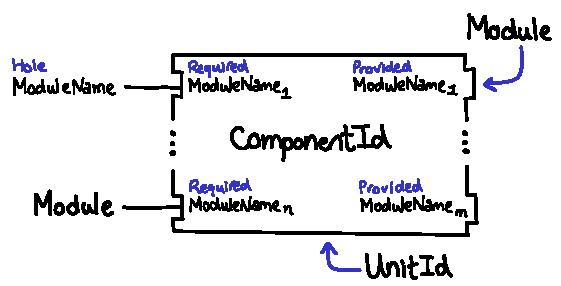
\includegraphics{figures/unit-identifier-pictorial.pdf}
\end{figure}

\noindent
Each component box is labelled with a component identifier and has a
series of input ports (on the left) and output ports (on the right). The
input ports represent all of the required module names of the component,
while the output ports signify a subset of the provided modules from
this component (output ports can be elided if they are unused). An
output port can be wired up to an input port to indicate the module is
being used to instantiate the requirement; if a ``hole'' module name is
wired to an input port, it indicates that this port is uninstantiated.
In our implementation of \Backpack{}, component graphs are acyclic
(but see Section~\ref{sec:recursive-uids} for the cyclic extension).

A unit identifier represents a specific box in a component graph, while
a module identifier represents a specific output port on one of these
boxes. It is worth emphasizing that the inputs to a component box
determine its identity: for example, the component box for a component
identifier can appear multiple times with different inputs.

Since \Backpack{} is an \emph{applicative} module system (functor
application is not generative), we can de-duplicate component boxes which
have the same component identifier and input modules, or (in reverse)
duplicate a component box and all of its inputs into two identical
graphs; in all of these cases, the diagrams represent multiple \uid{}s
which share common sub-expressions.  For example, the following
two diagrams are equivalent.

\begin{figure}[H]
\center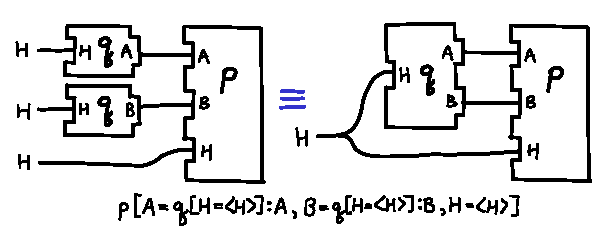
\includegraphics{figures/unit-identifier-pictorial-equivalence-example-2.pdf}
\end{figure}

The most expanded representation is always a tree of component boxes, each
with only a single output port; this representation corresponds exactly
to the abstract syntax tree of unit identifiers:

\begin{figure}[H]
\center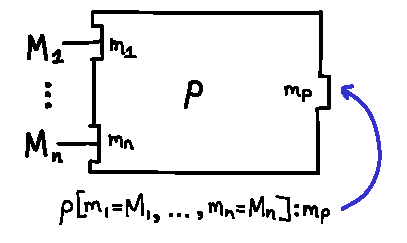
\includegraphics{figures/module-identifier-pictorial.pdf}
\end{figure}

\section{Substitutions}

Module substitutions can be applied to both unit and module identifiers, treating hole
modules as variables:

\[
\begin{array}{rcl}
  \substw{(\icid{p}{S})}{S'} &=_P& \icid{p}{\substw{S}{S'}} \\
  \\
  \substw{\holevar{m}}{\cdot} &=_M& \holevar{m} \\
  \substw{\holevar{m}}{\subst{m}{M}, S} &=_M& M \\
  \substw{\holevar{m}}{\subst{m'}{M}, S} &=_M& \substw{\holevar{m}}{S} \quad (m \neq m') \\
  \substw{(\Mod{P}{m})}{S} &=_M& \Mod{\substw{P}{S}}{m} \\
  \\
  \substw{(\overline{\subst{m}{M}})}{S} &=_{S}& \overline{\subst{m}{\substw{M}{S}}} \\
\end{array}
\]

\noindent
Pictorially, substitution plugs a component into an unfilled
hole module:

\begin{figure}[H]
\center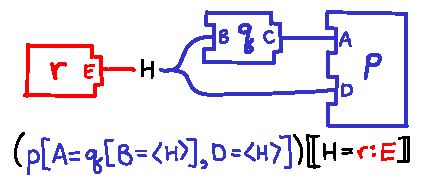
\includegraphics{figures/substitution-pictorial-example.pdf}
\end{figure}

